%\ihead{\headmark}
\chapter{Visualization}


\makeatletter
\renewcommand{\@chapapp}{}% Not necessary...
\newenvironment{chapquote}[2][2em]
{\setlength{\@tempdima}{#1}%
	\def\chapquote@author{#2}%
	\parshape 1 \@tempdima \dimexpr\textwidth-2\@tempdima\relax%
	\itshape}

\makeatother

\begin{center}
\begin{chapquote}{}
	``A picture is worth a thousands words.''
\end{chapquote}
\end{center}

Raw numbers to the users do not make sense and therefore, require necessary tools to display the result. Visualization allows us to see the broader aspects of complex data by showing the data in graphical formats. It really helps in capturing the user's attention and engage him through out the process. Complex data that could easily be ignored, can still be recognized and captured the attention of the user in a graphical reports \cite{quora:Sulakshana}.

The visualization tool Grafana has been set up for displaying the real-time data received from the sensors. All devices send the data in real-time which first get stored in Influxdb and then Grafana tool loads the data from there and display it on the graph. 

\section{Grafana}
Grafana is an open source real-time visualization tool for analytics and monitoring. It is one of the best tools for time series analytics, therefore, it is used for visualizing the real-time graphs from sensor devices. It can be used for any kind of application analytics, for example, industrial sensors, home automation, hospitals, weather reports etc. It allows to connect to many data sources available and pull data from it to do the analytics or the visualization. The most commonly used data sources these days are:

\begin{itemize}
	\item Elasticsearch
	\item InfluxDB
	\item Graphite
	\item Prometheus  
\end{itemize}

It allows us to connect to these data sources on just few click which makes it very convenient. Multiple dashboards can be created in Grafana to view different dimensions of the data. It also provides multiple tools for creating graphs in different fashion and styles which can be added to dashboards.

\section{InfluxDB}
 Since the sensor data is always time critical, therefore, a time series database is required for storing the data. InfluxDB is one of the best time series database available, therefore, it has been chosen for storing the sensors data. 
 
 It is very easy install and manage, and does not require other dependencies to run. It also provides an HTTP/HTPPS interface to read and write data from the database. The retention policy can be set on the database to manage space conveniently. The basic terms in InfluxDB are:
 
 \begin{itemize}
 	\item Database name
 	\item Measurement (same as table name in traditional databases)
 	\item Tags (to filter data)
 	\item Fields (actual data values)
 \end{itemize}
 
 The fields are generally used in a key value pair, with a timestamp field. Only one point can be stored at any specific timestamp. The precision of a single field can be in s, ms, $\mu$s, ns. If the field does not contains a timestamp field, then InfluxDB will generate a timestamp automatically.
 
 
 \section{Setting up Grafana with InfluxDB}
 Another reason for choosing the InfluxDB is that, it is really easy to configure Grafana for using InfluxDB as a data source. It is so simple that, the setup can be done in just 5 minutes. First, a user needs to create a database in the InfluxDB. Once the database is ready, starts the Grafana server. Generally, it runs on port 3000 but because of ports conflict, it is recommended to change the port to some other address by editing the \textit{conf\textbackslash sample.ini} file.
 
 
 Once the server is started, go to \textit{localhost:3000} address to open the Grafana web interface. Select an option to add a new data source. Lets say the database name is ``medit'', then configure the InfluxDB data source as shown in figure \ref{fig:gr_db_setup}.
 
 \begin{figure}[htpb]
 	\centering
 	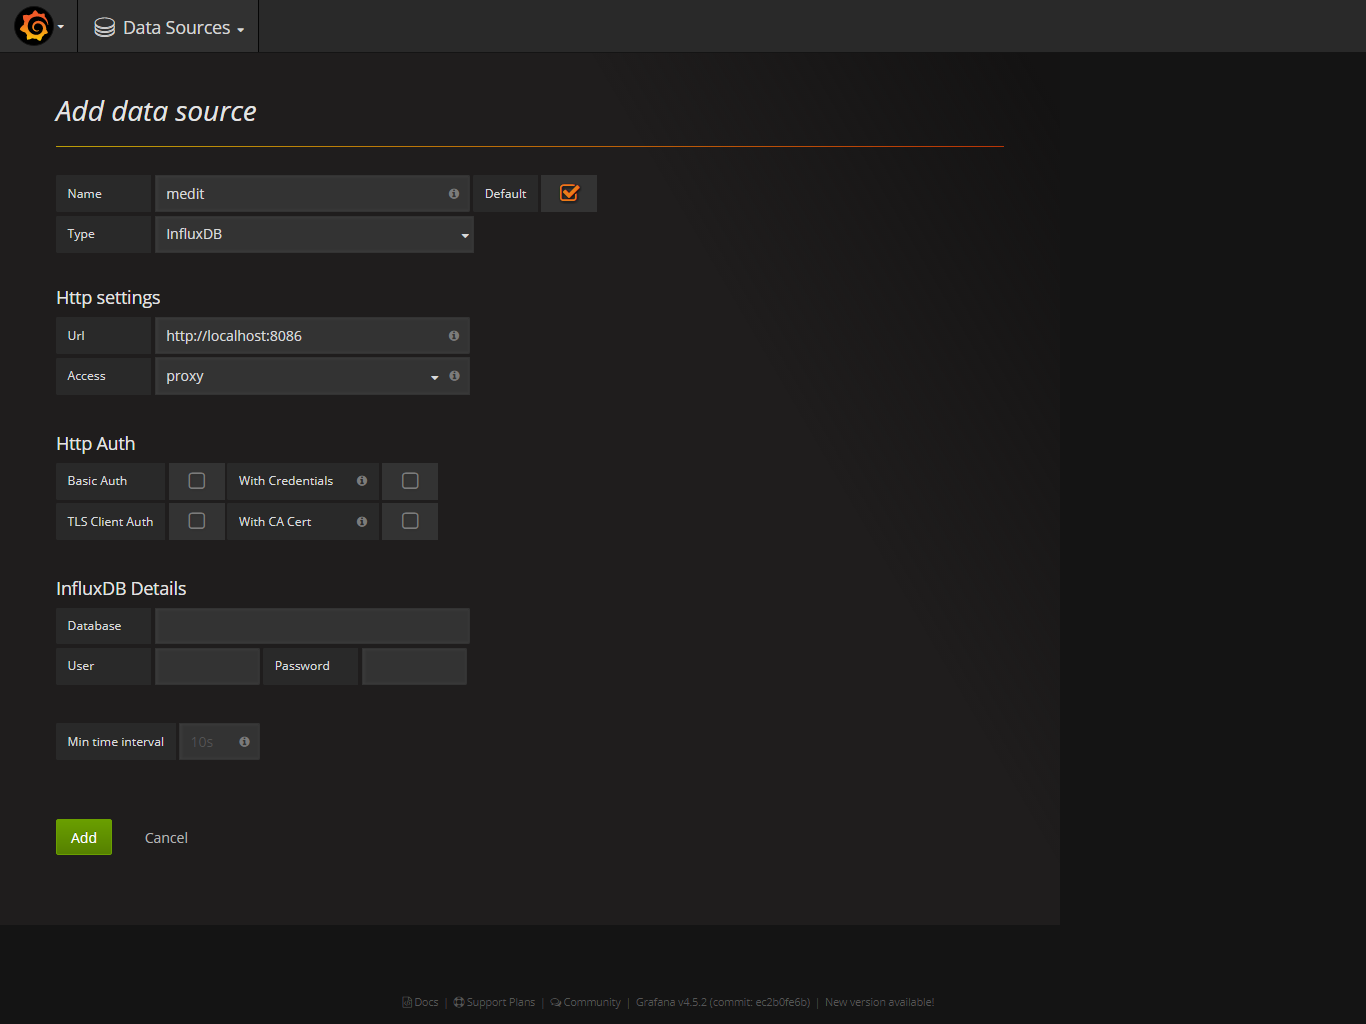
\includegraphics[width=16cm,height=15cm,keepaspectratio=true]{images/gr_db_setup}
 	\caption{
 		InfluxDB data source setup in Grafana.
 	}
 	\label{fig:gr_db_setup}
 \end{figure}



 \begin{figure}[htpb]
	\centering
	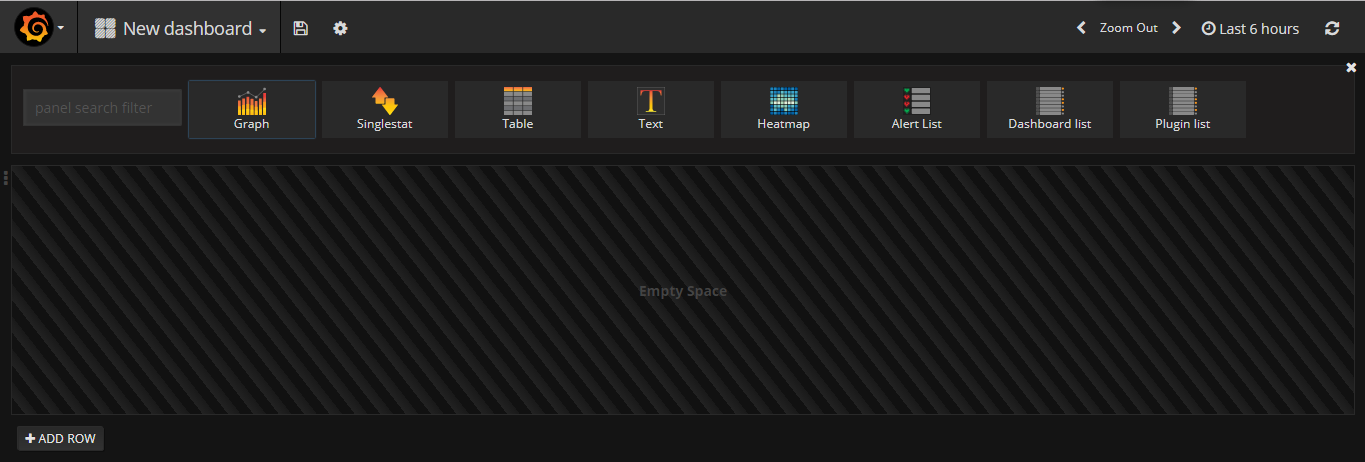
\includegraphics[width=16cm,height=15cm,keepaspectratio=true]{images/dashboard}
	\caption{
		Dashboard setup.
	}
	\label{fig:dashboard}
\end{figure}

Once the data source is setup, a dashboard is created to add the graphs and panels where the data is visualized. Multiple types of panels are available by default such as table, graphs, text, single stat, alert list, etc.

Lets say a graph is added to the dashboard. Now, a data source is need to be defined for the graph. That can be done by selecting the graph and edit it. The interface for setting up the data source for graph can be seen in figure \ref{fig:gr_query}. A very user-friendly interface is available where one can define a query for the panel. A query can be build just by selecting the option from drop down. It will contains all the information from the database that is setted up in the data source, that shown in figure \ref{fig:gr_db_setup}. So user simply needs to select the data source, then from the measurements select the specific measurement that wants to be chosen. One measurement can have multiple fields therefore, select a specific field which needs to be displayed on graph. Once all the steps are done, the panel is ready to display the information from the InfluxDB.


 \begin{figure}[htpb]
	\centering
	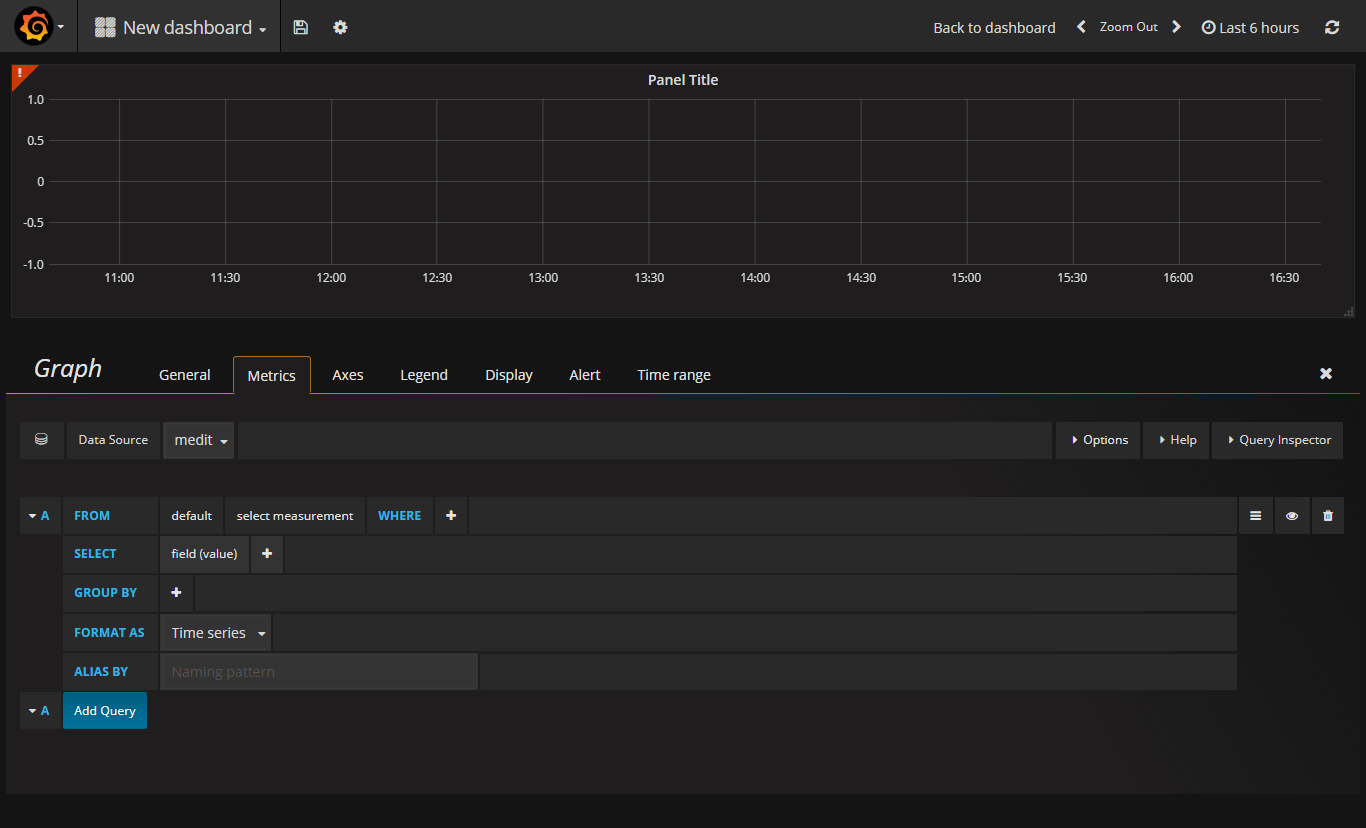
\includegraphics[width=16cm,height=15cm,keepaspectratio=true]{images/gr_query}
	\caption{
		Interface to add query for the panel.
	}
	\label{fig:gr_query}
\end{figure}


\section{Lambda Architecture for Big Data Processing}
The amount of data being processed nowadays is enormous, and this is often coined as Big Data. Big data is everywhere in the form of web logs, events, social networks, sensors data,etc, and these all are generating around petabytes of data each day. And because of this humongous amount of data, the traditional tools and storage technologies are unable to handle and cope with it. Therefore, this has led to a technology phase shift how we keep and manage our data, and to the development of Advance Analytics solutions.

Lambda Architecture \cite{UBDLAH} \cite{oreillyla} \cite{7364082} \cite{maprla} is getting involved in machine learning and data science applications day by day by enabling the real-time data processing and analytics without using the traditional ETL approach. It is designed to address the fault-tolerance, scalability and robustness issues of big data systems. Moreover, Lambda Architecture also ensure the low-latency and accuracy of the result. It combines the power of stream processing with batch processing to provide such kind of system.
Lambda architecture, as shown in figure \ref{fig:lambda_arc}, consists of 3 main components:


\begin{enumerate}
	\item Speed Layer
	\item Batch Layer
	\item Serving Layer
	
\end{enumerate}


\begin{figure}[htpb]
	\centering
	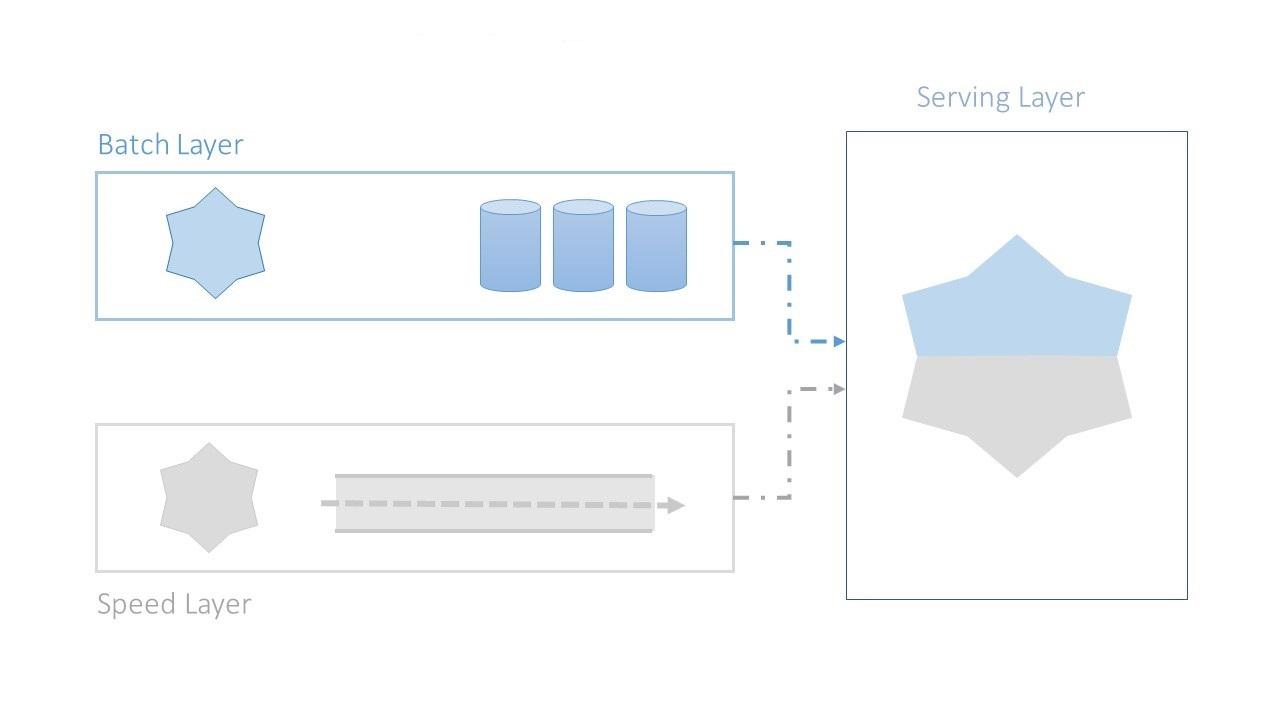
\includegraphics[width=12cm,height=10cm,keepaspectratio=true]{images/lambda_arc}
	\caption{
		Basic supervised machine learning workflow.
	}
	\label{fig:lambda_arc}
\end{figure}



\subsection{Batch Layer}
The Batch layer will hold all of the master data which will be stored in Apache Hadoop. This data will be kept in its original state, untouched and in an immutable manner. This data will be processed and generate the batch views which then will be served in the serving layer. This is the place which will provide the most accurate results from the data using any of the available distributed platform tools.

\subsection{Speed Layer}
Typically, it is known that a Hadoop processing frameworks are slow and take a lot of time. To cope up with this problem, Lambda Architecture introduces the speed layer. Speed layer process the real-time stream and generate the real-time views of a short time frame, which are then serve in a serving layer along with batch views. The main point to notice here is that the speed layer data is temporal in nature, i.e. it can only store that much amount of data that could be kept in the memory. And it is deleted as soon as one batch process is completed.

\subsection{Serving Layer}
This is a place where the final results and data are visualized. Serving layer provides an interface which integrates real-time views with batch views and unified them together. An accurate view of data will be presented by the batch layer, whereas the fresh view of the data will be presented by the speed layer. It also supports ad-hoc queries which are optimized for low-latency. Technologies which can be used in this layers are Cassandra, HBase, etc.

The data source will provide the data which will be streamed in the stream layer and at the same time to the batch layer. Batch layer will hold the data for a long time and stream layer will process the stream in a window of short time and then provide the calculated result. The serving layer will combine the data received from the batch layer, more specifically the batch views, and the data received from the speed layer and allow them to query from a single interface. The advantage of the Lambda Architecture is that if one layer is down, the other layer can be used to make system available. For example, in figure \ref{lambda_arc_1}, if a speed layer is down, which of course can happen in the production environment, The batch layer can be used to compensate the failure.


\begin{figure}[htpb]
	\centering
	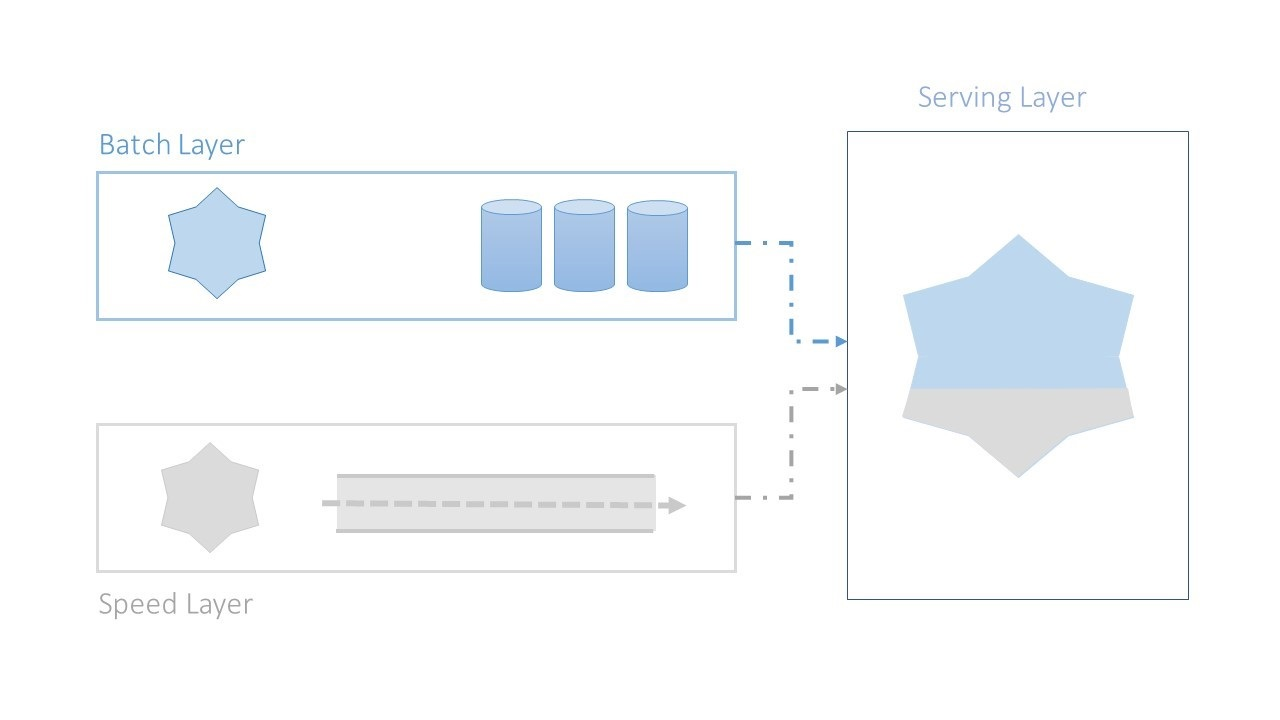
\includegraphics[width=12cm,height=10cm,keepaspectratio=true]{images/lambda_arc_1}
	\caption{
		Basic supervised machine learning workflow.
	}
	\label{fig:lambda_arc_1}
\end{figure}

The reason why it is called lambda architecture is because the lambda symbol splits into two parts which in case of this architecture represents the batch layer and the speed layer. 

\begin{figure}[htpb]
	\centering
	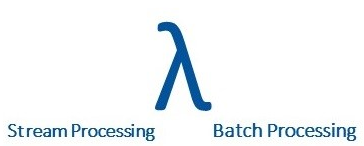
\includegraphics[width=12cm,height=10cm,keepaspectratio=true]{images/lambda_new}
	\caption{
		Basic supervised machine learning workflow.
	}
	\label{fig:lambda}
\end{figure}

Typically, the data stream is implemented using a publish-subscribe messaging system such as Kafka, which can easily scale for high velocity data ingestion. It can be thought of as a place where publishers publish their data and the consumers read data from it. This is different from the traditional queue as it keeps the data until we let it to hold. In contrast, the data will be removed from the queue, once it is delivered to the appropriate consumer of the data. It uses topics to publish and to subscribe for the data. Every Kafka server is known as broker and since it is a distributed system, therefore, there can be more than one broker. The more the number of brokers are, the higher the availability is. The advantage of having Kafka is that it can handle many different forms of data, such as sensors data, application events, server logs, social network events etc. Kafka is very fast despite of having heavy load.

\begin{figure}[htpb]
	\centering
	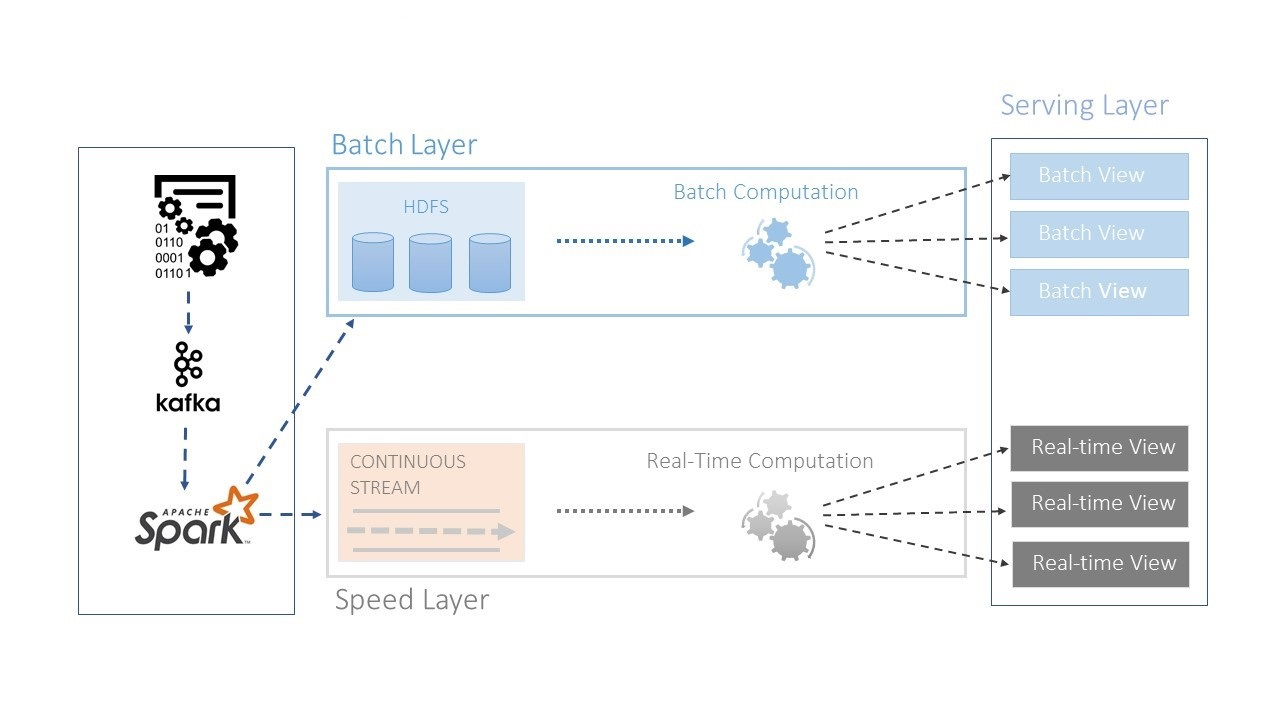
\includegraphics[width=17cm,height=15cm,keepaspectratio=true]{images/imp_lambda_arc}
	\caption{
		Basic supervised machine learning workflow.
	}
	\label{fig:impl_lambda_arc}
\end{figure}


The implementation of lambda architecture has been shown in figure \ref{fig:impl_lambda_arc}. The data will directly be published from data source to Kafka based on some topic. Data from multiple data sources can be collected via Kafka based on different topic names. Once the data is fed into the Kafka, the corresponding consumers will read the data from Kafka using the topic name where the data publish to. In this architecture, Apache Spark can be used in both the batch layer and the speed layer. 

Apache Spark is a large-scale data processing tool, which runs 100 times faster than the Hadoop MapReduce by caching the data objects in the memory. Thus, it is a strong candidate to replace the MapReduce. It also creates a lineage graph. So, in case of failure, it can do the computations again and go back to the last state of the data. These are two of the fundamental things that Resilient Distributed Data Set (RDD) is all about. It is specially designed to schedule and execute a large amount of data. Apache Spark does not only provide the batch processing, but it also comes with real-time stream processing, machine learning tools, graph processing, Spark SQL, Spark R and complex analytics. It is designed to run everywhere, such as it can run on Hadoop YARN, apache Mesos or standalone as well. Apache Spark offers interface for several languages to write the applications. The available languages are Java, Scala, Python and R.
